\documentclass[11pt]{article}

% ---------- Packages ----------
\usepackage[margin=1in]{geometry}
\usepackage{times}
\usepackage[T1]{fontenc}
\usepackage{graphicx}
\usepackage{booktabs}
\usepackage{array}
\usepackage{amsmath}
\usepackage{amssymb}
\usepackage{xcolor}
\usepackage{hyperref}
\usepackage{titlesec}
\usepackage{enumitem}
\usepackage{caption}
\usepackage{fancyhdr}
\usepackage{multirow}
\usepackage{tabularx}

% ---------- Colors ----------
\definecolor{navy}{HTML}{123B4F}
\definecolor{teal}{HTML}{1B7A72}
\definecolor{coral}{HTML}{D9614F}

% ---------- Hyperref setup ----------
\hypersetup{
    colorlinks=true,
    linkcolor=teal,
    citecolor=teal,
    urlcolor=teal,
    pdftitle={Micro-Q-Instruct: A Degradation-Aware Microscopy Benchmark},
    pdfauthor={Shayan Salehi, Ali Hezaveh}
}

% ---------- Section styling ----------
\titleformat{\section}
  {\Large\bfseries\color{navy}}{\thesection}{0.6em}{}
\titleformat{\subsection}
  {\large\bfseries\color{teal}}{\thesubsection}{0.6em}{}

% ---------- Header/footer ----------
\pagestyle{fancy}
\fancyhf{}
\renewcommand{\headrulewidth}{0.4pt}
\fancyhead[L]{\small Micro-Q-Instruct}
\fancyhead[R]{\small DIP Final Project}
\fancyfoot[C]{\small\thepage}

\setlength{\parskip}{0.5em}
\setlength{\parindent}{0pt}

\title{\vspace{-1.5cm}\textbf{\color{navy}Micro-Q-Instruct}\\[0.3em]
\large A Degradation-Aware Microscopy Benchmark: From Controlled Classical Image Processing to Paired Vision-Language Model Robustness}
\author{Shayan Salehi (404203509) \and Ali Hezaveh (404208531)}
\date{Department of Computer Engineering, Sharif University of Technology\\
Digital Image Processing Course \,--\, Final Project\\
Instructor: Prof. Kasaei}

\begin{document}

\maketitle
\thispagestyle{fancy}

\begin{abstract}
\noindent
Vision-language models (VLMs) increasingly encounter microscopy images through
acquisition pipelines that introduce blur, noise, sub-sampling, compression, and
detector artifacts. A model's semantic answer about a specimen may depend on this
low-level acquisition quality just as much as on biological content, yet natural-image
quality benchmarks rarely model microscopy physics, and microscopy-focused VLM
benchmarks rarely isolate low-level corruption. This project, \emph{Micro-Q-Instruct},
addresses that gap with a traceable, paired benchmark in which every corruption and
restoration step is known and reproducible. Starting from 1{,}701 clean microscopy
sources drawn from permissive training/development pools and the pinned, official
$\mu$-Bench evaluation set, we generate 15{,}480 degradation recipes spanning ten
physically motivated degradation families at three severity levels, producing 30{,}960
paired derivatives (degraded and restored). Each image is characterized by a
19-feature classical fingerprint and scored with paired fidelity metrics (MSE, PSNR,
SSIM, edge retention, histogram divergence). A matched classical restoration strategy
is applied per family, and 99.95\% of eligible severity triplets are verified to be
PSNR-monotonic. In a second phase, we stress-test Qwen3-VL-8B on 500 unique paired
Micro-Bench samples across clean, degraded, and restored image conditions while
holding the question, options, model, prompt, and decoding parameters fixed. We find
that restoration recovers most, but not all, of the aggregate semantic robustness loss
(66.8\%~$\to$~65.2\%~$\to$~66.4\% macro accuracy), that recovery is strongly
family-dependent (periodic interference: $-12.9$~pp degradation loss, $+11.5$~pp
restoration gain; photobleaching and quantization remain information-limited), and
that fine-grained perception tasks are the primary stress point under strong
corruption. The result is a reproducible, audit-tracked classical DIP benchmark
coupled with an inference-time robustness study that connects pixel-level image
quality to downstream VLM correctness.
\end{abstract}

\tableofcontents
\newpage

% ============================================================
\section{Introduction and Motivation}
% ============================================================

Vision-language models are increasingly used to interpret microscopy images for
tasks ranging from coarse modality recognition to fine-grained morphological
reasoning. However, a VLM does not see the specimen directly --- it sees the
specimen \emph{through an acquisition pipeline}. A correct semantic answer may
depend on blur, noise, sampling, compression, registration, and detector response,
not solely on biological content.

This motivates the central question addressed by this project: \emph{does image
quality belong in microscopy reasoning benchmarks, and if so, how should it be
measured?} Two lines of prior work are relevant but insufficient on their own:

\begin{itemize}[leftmargin=1.4em]
    \item Natural-image quality benchmarks (e.g., low-level vision curricula such as
    Q-Instruct and Q-Bench) rarely model microscopy-specific physics such as
    Poisson-Gaussian shot noise, photobleaching, or PSF-governed defocus.
    \item Microscopy-focused VLM benchmarks (e.g., $\mu$-Bench) evaluate semantic and
    biological reasoning but rarely isolate low-level image corruption as an
    independent, controlled variable.
\end{itemize}

Our response is a \textbf{traceable, paired benchmark} in which every corruption and
every restoration is known: exact parameters, random seeds, bit depth, content
hashes, and source licenses are recorded for every generated image, so quality
$\to$ evidence $\to$ answer can be audited end to end.

\subsection{Research Questions}

The project is organized around three research questions, all evaluated on a shared,
paired experimental spine in which \emph{only the pixels change} --- the question,
answer options, correct answer, model, prompt template, and decoding parameters are
held fixed:

\begin{enumerate}[leftmargin=1.6em]
    \item \textbf{Detect.} Can an interpretable digital image processing (DIP)
    fingerprint identify degradation family and severity across heterogeneous
    microscopy domains (fluorescence, light, electron)?
    \item \textbf{Restore.} Which matched classical restoration method recovers
    fidelity, edge content, and morphology for each degradation family --- and where
    is information irreversibly lost?
    \item \textbf{Stress-test.} Does a modern VLM (Qwen3-VL) preserve the same correct
    answer across clean, degraded, and restored views of the same image?
\end{enumerate}

\subsection{Course Alignment}

The project was designed so that essentially every chapter of the Digital Image
Processing syllabus becomes an implemented, measurable artifact rather than a purely
theoretical exercise. Table~\ref{tab:syllabus} summarizes this mapping.

\begin{table}[h]
\centering
\small
\begin{tabularx}{\linewidth}{@{}l l X@{}}
\toprule
\textbf{Chapter} & \textbf{Topic} & \textbf{Implemented artifact} \\
\midrule
Ch. 2 & Digital fundamentals & Sampling, anti-aliasing, quantization, pixel precision \\
Ch. 3 & Spatial processing & PSF modeling, gradients, Laplacian, gamma, CLAHE \\
Ch. 4 & Frequency domain & Spectral energy, sinusoidal interference, notch rejection \\
Ch. 5 & Restoration & Poisson/read noise modeling, local Wiener filtering, deconvolution \\
Ch. 7 & Transforms & Wavelet energy fingerprints and denoising \\
Ch. 8 & Compression & Controlled JPEG and block-boundary evidence \\
Ch. 9 & Morphology & Otsu proxy masks, Dice/IoU, connected components \\
Bridge & Vision-language robustness & Paired inference, uncertainty, exact-answer scoring \\
\bottomrule
\end{tabularx}
\caption{Mapping of DIP course chapters to implemented components of the benchmark.
Foundational references: $\mu$-Bench (NeurIPS 2024), Q-Instruct (CVPR 2024), Q-Bench
(ICLR 2024).}
\label{tab:syllabus}
\end{table}

% ============================================================
\section{Project Overview: A Two-Phase Causal Chain}
% ============================================================

The pipeline is structured as a causal chain that moves from raw microscopy images
to robustness evidence:

\[
\text{Clean microscopy} \;\rightarrow\; \text{Controlled degradation} \;\rightarrow\;
\text{DIP fingerprint} \;\rightarrow\; \text{Matched restoration} \;\rightarrow\;
\text{Paired VLM test}
\]

\textbf{Phase 1 --- Classical DIP benchmark.} Produces paired images, exact generation
recipes, interpretable per-image measurements, morphology metrics, restored images, and
a classical restoration baseline. This phase involves no learned model and is fully
deterministic given a master random seed.

\textbf{Phase 1.5 --- Inference-time robustness.} Measures answer stability of a
vision-language model (Qwen3-VL) with paired statistics across the clean / degraded /
restored conditions. No model training or fine-tuning occurs in this phase; it is a
pure evaluation study.

% ============================================================
\section{Phase 1: Data Sourcing and Integrity}
% ============================================================

\subsection{Strict Two-Pool Policy}

To avoid any contamination between data used for calibrating the pipeline and data used
for reporting final numbers, the project enforces a strict train/evaluate separation:
classical strategies and thresholds are tuned on permissive external sources, while all
reported evaluation numbers come exclusively from the pinned, official $\mu$-Bench
evaluation set.

From 1{,}701 unique clean source images, the pipeline allocates:

\begin{itemize}[leftmargin=1.4em]
    \item \textbf{804} images to \textit{training} (external sources such as BBBC010,
    BBBC038, IDR0067);
    \item \textbf{147} images to \textit{development}, held out purely for calibration;
    \item \textbf{750} images to \textit{evaluation}, drawn from 15 official $\mu$-Bench
    datasets, with the $\mu$-Bench revision pinned to commit \texttt{3f2c5b59\ldots}.
\end{itemize}

The modality composition of the pool is fluorescence-heavy but multi-modal: 893
fluorescence, 625 light microscopy, and 183 electron microscopy images. All records
retain their original license (CC0, CC0-1.0, CC-BY-4.0, or CC-BY-SA-4.0). A
\textbf{contamination guard} combines decoded-pixel SHA-256 hashing, a 64-bit
perceptual-hash nearest-neighbor audit, and a license allowlist to ensure no evaluation
image leaks into the training or development pools.

\subsection{Balanced, Deterministic Degradation Planning}

Rather than applying every degradation family to every image (a full factorial design),
the pipeline uses a \textbf{balanced incomplete factorial}: for each clean source, nine
variants are generated by selecting three physically applicable degradation families and
combining each with weak, medium, and strong severity. Deterministic clean controls and
a configured fraction of mixed (stacked) corruptions are added on top of this design.
The entire generation process is seeded with a single master seed
(\texttt{20260724}), making every recipe exactly reproducible.

Applicability is \textbf{physics-aware}: for example, photobleaching and channel-shift
degradations are restricted to fluorescence images; chromatic misregistration requires
genuinely multichannel content; and defocus blur is restricted to optical (light and
fluorescence) modalities. Degradation parameters additionally scale with image size so
that severity is comparable across differently sized sources.

This design yields:
\begin{itemize}[leftmargin=1.4em]
    \item \textbf{10} degradation families,
    \item \textbf{3} severity levels (weak / medium / strong),
    \item \textbf{15{,}480} degraded images,
    \item \textbf{15{,}480} matched restored images,
    \item \textbf{30{,}960} total paired derivatives.
\end{itemize}

Every recipe preserves full provenance: image role (train/dev/eval), exact
degradation and restoration parameters, random seed, bit depth, SHA-256 content hash,
source license, and output path.

% ============================================================
\section{Phase 1: The Ten Degradation Families}
% ============================================================

Each degradation family is implemented as a physically motivated forward model with a
matched classical restoration strategy. Representative results at \textbf{strong}
severity are summarized below, with paired image evidence (PSNR, SSIM, and their
restoration deltas $\Delta$PSNR, $\Delta$SSIM).

\begin{table}[h]
\centering
\small
\begin{tabularx}{\linewidth}{@{}l X X@{}}
\toprule
\textbf{Family} & \textbf{Degradation model} & \textbf{Matched restoration} \\
\midrule
1. Sampling / resolution loss &
Downsample then reconstruct at original dimensions, removing spatial samples and
exposing aliasing/blur. &
BayesShrink db2 wavelet denoising (artifact suppression only; removed samples are not
invertible). \\
2. Bit-depth quantization &
Uniform intensity quantization collapses the continuous tonal range into a small set of
discrete levels. &
Wavelet denoising softens contouring but cannot recreate discarded intensity levels. \\
3. Poisson--Gaussian noise &
Photon-count shot noise combined with additive read noise to mimic noisy acquisition. &
Local adaptive Wiener filter using neighborhood statistics to attenuate signal-dependent
noise. \\
4. Defocus blur &
Normalized disk point-spread function (PSF) removes high-frequency focus cues. &
Recorded-PSF Wiener deconvolution, trading sharpness against ringing/noise
amplification. \\
5. Motion / scan drift &
Normalized linear PSF smears structures along a controlled length and angle. &
Recorded linear-PSF Wiener deconvolution, partially reconstructing edge direction and
texture. \\
6. Periodic interference &
Oriented sinusoid adds coherent striping at a known spatial frequency and amplitude. &
Paired notch-reject filter removing the synthetic frequency peaks (an explicitly
oracle-assisted baseline). \\
7. JPEG compression &
Lossy block-transform coding discards coefficients, introducing block/ringing
artifacts; 16-bit inputs also incur an 8-bit round trip. &
Wavelet denoising smooths post-compression artifacts, but discarded coefficients remain
unrecoverable. \\
8. Photobleaching &
Fluorescence signal is attenuated above background (models retained intensity, not
detector clipping). &
Gamma correction plus CLAHE restores visibility/local contrast without recreating lost
photons. \\
9. Chromatic misregistration &
Opposing subpixel channel shifts create color fringes in multichannel fluorescence
images. &
Phase-correlation channel registration estimates displacement relative to the green
channel and realigns red/blue. \\
10. Detector saturation &
Gain and black-level changes followed by detector-range clipping, flattening bright
structures. &
Gamma/CLAHE enhancement redistributes visible contrast; clipped values cannot be
reconstructed. \\
\bottomrule
\end{tabularx}
\caption{The ten degradation families, their forward (degradation) models, and their
matched classical restoration strategies.}
\label{tab:families}
\end{table}

% ============================================================
\section{Phase 1: Measurement and Restoration Framework}
% ============================================================

\subsection{19-Feature Interpretable Fingerprint}

Every image (clean, degraded, and restored) is characterized by a 19-dimensional
classical feature vector, deliberately chosen to be interpretable rather than learned:
histogram statistics, entropy, gradient and Laplacian energy, Fourier band-energy
ratios, spectral centroid, wavelet sub-band energy, blockiness, clipping fraction, and
inter-channel shift.

\subsection{Paired Image Evidence}

For every degraded/restored pair relative to its clean reference, the pipeline computes:
\begin{itemize}[leftmargin=1.4em]
    \item pixel-fidelity metrics: MSE, PSNR, SSIM;
    \item structural metrics: edge-retention ratio, histogram Jensen--Shannon
    divergence;
    \item where segmentation masks exist: Dice coefficient, IoU, region area, and
    connected-component counts (via Otsu proxy masks).
\end{itemize}

\subsection{Restoration Strategy Registry}

A registry of six classical restoration strategies is applied per family according to
the matching in Table~\ref{tab:families}: local Wiener filtering, PSF-aware
deconvolution, frequency-domain notch rejection, phase-correlation channel
registration, gamma correction with CLAHE, and wavelet-domain comparison/denoising.

\subsection{Release Validation}

The full Phase 1 release comprises \textbf{15{,}480} materialized recipes generated
from \textbf{1{,}701} clean source images, split into \textbf{7{,}327} training,
\textbf{6{,}822} evaluation, and \textbf{1{,}331} development records. Validation of the
release reports \textbf{zero errors and zero warnings} across all 15{,}480 analyses,
and \textbf{3{,}743 of 3{,}745} eligible severity triplets (99.95\%) satisfy strict PSNR
monotonicity, i.e.\ $\mathrm{PSNR}(\text{weak}) \geq \mathrm{PSNR}(\text{medium}) \geq
\mathrm{PSNR}(\text{strong})$. The release package includes recipe / generated /
restored JSONL manifests, paired CSV and JSONL analysis records, a dataset card, an
audit log, validation and calibration figures, and serialized classical baselines.

% ============================================================
\section{Phase 1: Results}
% ============================================================

\subsection{Feature Space Heterogeneity}

Exploratory analysis of the 19-feature fingerprint across the full dataset shows that
microscopy images span radically different visual regimes. The entropy distribution is
broad and multimodal, with low-information fields (e.g.\ sparse fluorescence puncta)
coexisting with richly textured brightfield specimens, so a single global threshold for
any detector would be brittle. Intensity variation (feature.intensity\_std) is strongly
right-skewed: most images have modest contrast, with a small high-contrast tail that
motivates per-modality normalization rather than a single global scale.

\subsection{Paired Fidelity Distributions}

Aggregate PSNR values concentrate in the 25--40~dB range but retain long tails in both
directions, reflecting the coexistence of subtle clean-control cases and destructive
strong corruptions. SSIM piles up near 1.0 while still spanning the full $[0,1]$ range,
confirming that PSNR and SSIM capture complementary failure modes and that neither
scalar alone summarizes degradation impact.

\subsection{Restoration Is Governed by Invertibility, Not Visual Polish}

Table~\ref{tab:restoration_delta} reports the mean evaluation-set restoration delta for
representative single-degradation families.

\begin{table}[h]
\centering
\small
\begin{tabular}{@{}l r r l@{}}
\toprule
\textbf{Family} & $\boldsymbol{\Delta}$\textbf{PSNR (dB)} & $\boldsymbol{\Delta}$\textbf{SSIM} & \textbf{Interpretation} \\
\midrule
Periodic interference & $+7.79$ & $+0.109$ & known-frequency notch filter excels \\
Poisson--Gaussian noise & $+5.21$ & $+0.165$ & local statistics are recoverable \\
Motion / scan drift & $+1.43$ & $+0.044$ & only partial PSF inversion possible \\
Bit-depth quantization & $-2.59$ & $-0.038$ & discarded levels cannot be regenerated \\
Photobleaching & $-12.11$ & $-0.274$ & contrast enhancement $\neq$ photon recovery \\
\bottomrule
\end{tabular}
\caption{Mean evaluation-set $\Delta$PSNR / $\Delta$SSIM after restoration for
selected single-degradation families. Positive values indicate the restoration
improves fidelity relative to the degraded image; negative values indicate that
classical enhancement further reduces measured fidelity even though it may
subjectively improve visibility.}
\label{tab:restoration_delta}
\end{table}

The key finding is that \textbf{restoration effectiveness tracks the invertibility of
the underlying forward model}, not the perceptual quality of the output. Degradations
with a known, structured forward operator (periodic interference, additive
signal-dependent noise, and to a lesser extent linear motion blur) are substantially
recoverable. Degradations that destroy information irreversibly --- discarded
quantization levels, clipped detector saturation, and attenuated fluorescence
signal --- cannot be recovered by contrast enhancement alone, and enhancement can even
\emph{reduce} measured pixel fidelity while improving apparent visibility.

As a secondary analysis, a simple cross-source linear classifier over the 19-feature
fingerprint was evaluated as a baseline degradation detector. It achieves 34.9\%
degradation-family accuracy (macro-F1 27.3\%) and 41.0\% severity accuracy (macro-F1
38.2\%). This confirms that classical features carry transferable signal about
degradation type and strength, but that cross-modality and cross-domain variation
prevents a simple linear fingerprint from becoming a universal, high-accuracy detector
--- motivating the more targeted, per-family restoration approach used elsewhere in the
pipeline.

\subsection{Severity Is Empirically Ordered but Not Equally Spaced}

Across all ten degradation families, 99.95\% of eligible paired severity triplets
satisfy $\mathrm{PSNR}(\text{weak}) \geq \mathrm{PSNR}(\text{medium}) \geq
\mathrm{PSNR}(\text{strong})$, confirming that the severity parameterization behaves
monotonically as intended. However, the weak$\to$medium$\to$strong slopes differ
substantially by family (e.g.\ chromatic misregistration and sampling loss degrade
gently, while quantization, Poisson--Gaussian noise, and detector saturation degrade
steeply), showing that severity must be calibrated per corruption type rather than
treated as a single universal physical scale.

% ============================================================
\section{Phase 1.5: Paired Inference-Time Robustness}
% ============================================================

\subsection{Experimental Design}

Phase 1.5 asks whether a vision-language model's semantic correctness on the official
$\mu$-Bench evaluation questions is preserved across the same three pixel conditions
used in Phase 1. For each unique sample (an evaluation image, its official multiple-choice
question, and one Phase-1 degradation recipe), three pixel conditions are constructed:

\begin{itemize}[leftmargin=1.4em]
    \item \textbf{Clean} --- the official $\mu$-Bench image, unmodified;
    \item \textbf{Degraded} --- the exact Phase 1 recipe applied to that image;
    \item \textbf{Restored} --- the matched restored image from Phase 1.
\end{itemize}

\textbf{Held constant} across all three conditions: the question text, answer options,
expected answer, prompt template, model, decoding parameters, and a sample-specific
random seed. \textbf{Changed deliberately}: only the image pixels. Prompts never reveal
which condition (clean, degraded, restored) is being shown, and request order is
deterministically shuffled to reduce order and load effects. The unit of analysis is the
independent image--question triplet; there is no pseudoreplication from asking multiple
questions about the same source image.

\subsection{Implementation}

The evaluation pipeline joins recipe, generated-image, restored-image, and official
annotation records by recipe ID; balances the sampled cohort across task type,
degradation family, severity, and modality (one question and one recipe per image); and
interleaves all three conditions in a deterministic, shuffled request order. Inference
is performed with \textbf{Qwen3-VL-8B} served via vLLM, using deterministic decoding and
a structured JSON answer request. Responses are parsed strictly by JSON field,
answer letter, index, or exact option text --- ambiguous responses are never guessed as
correct.

The resulting cohort comprises \textbf{500} unique paired samples (167 coarse-perception
and 333 fine-perception questions; 100 electron, 100 fluorescence, and 300 light
microscopy samples), yielding \textbf{1{,}500} completed inference requests across
\textbf{6} perception task types, with a \textbf{100\%} answer-parse rate.

\subsection{Statistical Methodology}

The primary endpoint is \textbf{task-macro accuracy},
\[
\mathrm{MacroAcc}(c) \;=\; \mathrm{mean}_{\text{task}}\;\mathrm{mean}_{\text{sample}}\;
\mathbb{1}\!\left[\hat{y}_{i,c} = y_i\right],
\]
where each of the six task types receives equal weight so that frequent task types
cannot dominate the aggregate score. Uncertainty is quantified with a 10{,}000-resample
paired bootstrap over complete image--question triplets, reporting 95\% percentile
confidence intervals. Condition-to-condition differences are additionally tested with
the exact McNemar test on discordant pairs, with Holm correction across the three
pairwise condition comparisons. Four paired effects are reported: degradation loss
(clean $\to$ degraded), restoration gain (degraded $\to$ restored), residual versus
clean (restored $\to$ clean), and recovery fraction. A full per-sample transition audit
classifies each triplet into one of eight categories (e.g.\ stable correct, restored
after failure, unrecovered failure, harmed by restoration).

It is important to note the \textbf{scope boundary} of this phase: the completed Phase 1
annotations only support coarse- and fine-perception question types; no higher-level
cognition category is inferred or fabricated for this analysis.

% ============================================================
\section{Phase 1.5: Results}
% ============================================================

\subsection{Overall Robustness}

Overall macro accuracy moves from \textbf{66.8\%} (clean) to \textbf{65.2\%} (degraded)
to \textbf{66.4\%} (restored) --- a $-1.62$ percentage-point (pp) degradation effect
followed by a $+1.21$~pp restoration gain. All three condition-level 95\% confidence
intervals overlap, so the aggregate effect is directionally consistent but not
individually significant at $n=500$.

Splitting by question granularity reveals a more informative pattern: \textbf{coarse
perception} accuracy (77.2\% $\to$ 78.4\% $\to$ 79.0\%) shows no consistent loss and, if
anything, a slight positive trend, whereas \textbf{fine perception} accuracy (61.6\%
$\to$ 58.6\% $\to$ 60.1\%) drops by \textbf{3.02~pp} under degradation and recovers only
\textbf{1.51~pp} with restoration --- confirming that fine-grained perceptual judgments
are considerably more sensitive to acquisition-level image quality than coarse,
modality-level judgments.

\begin{figure}[h]
    \centering
    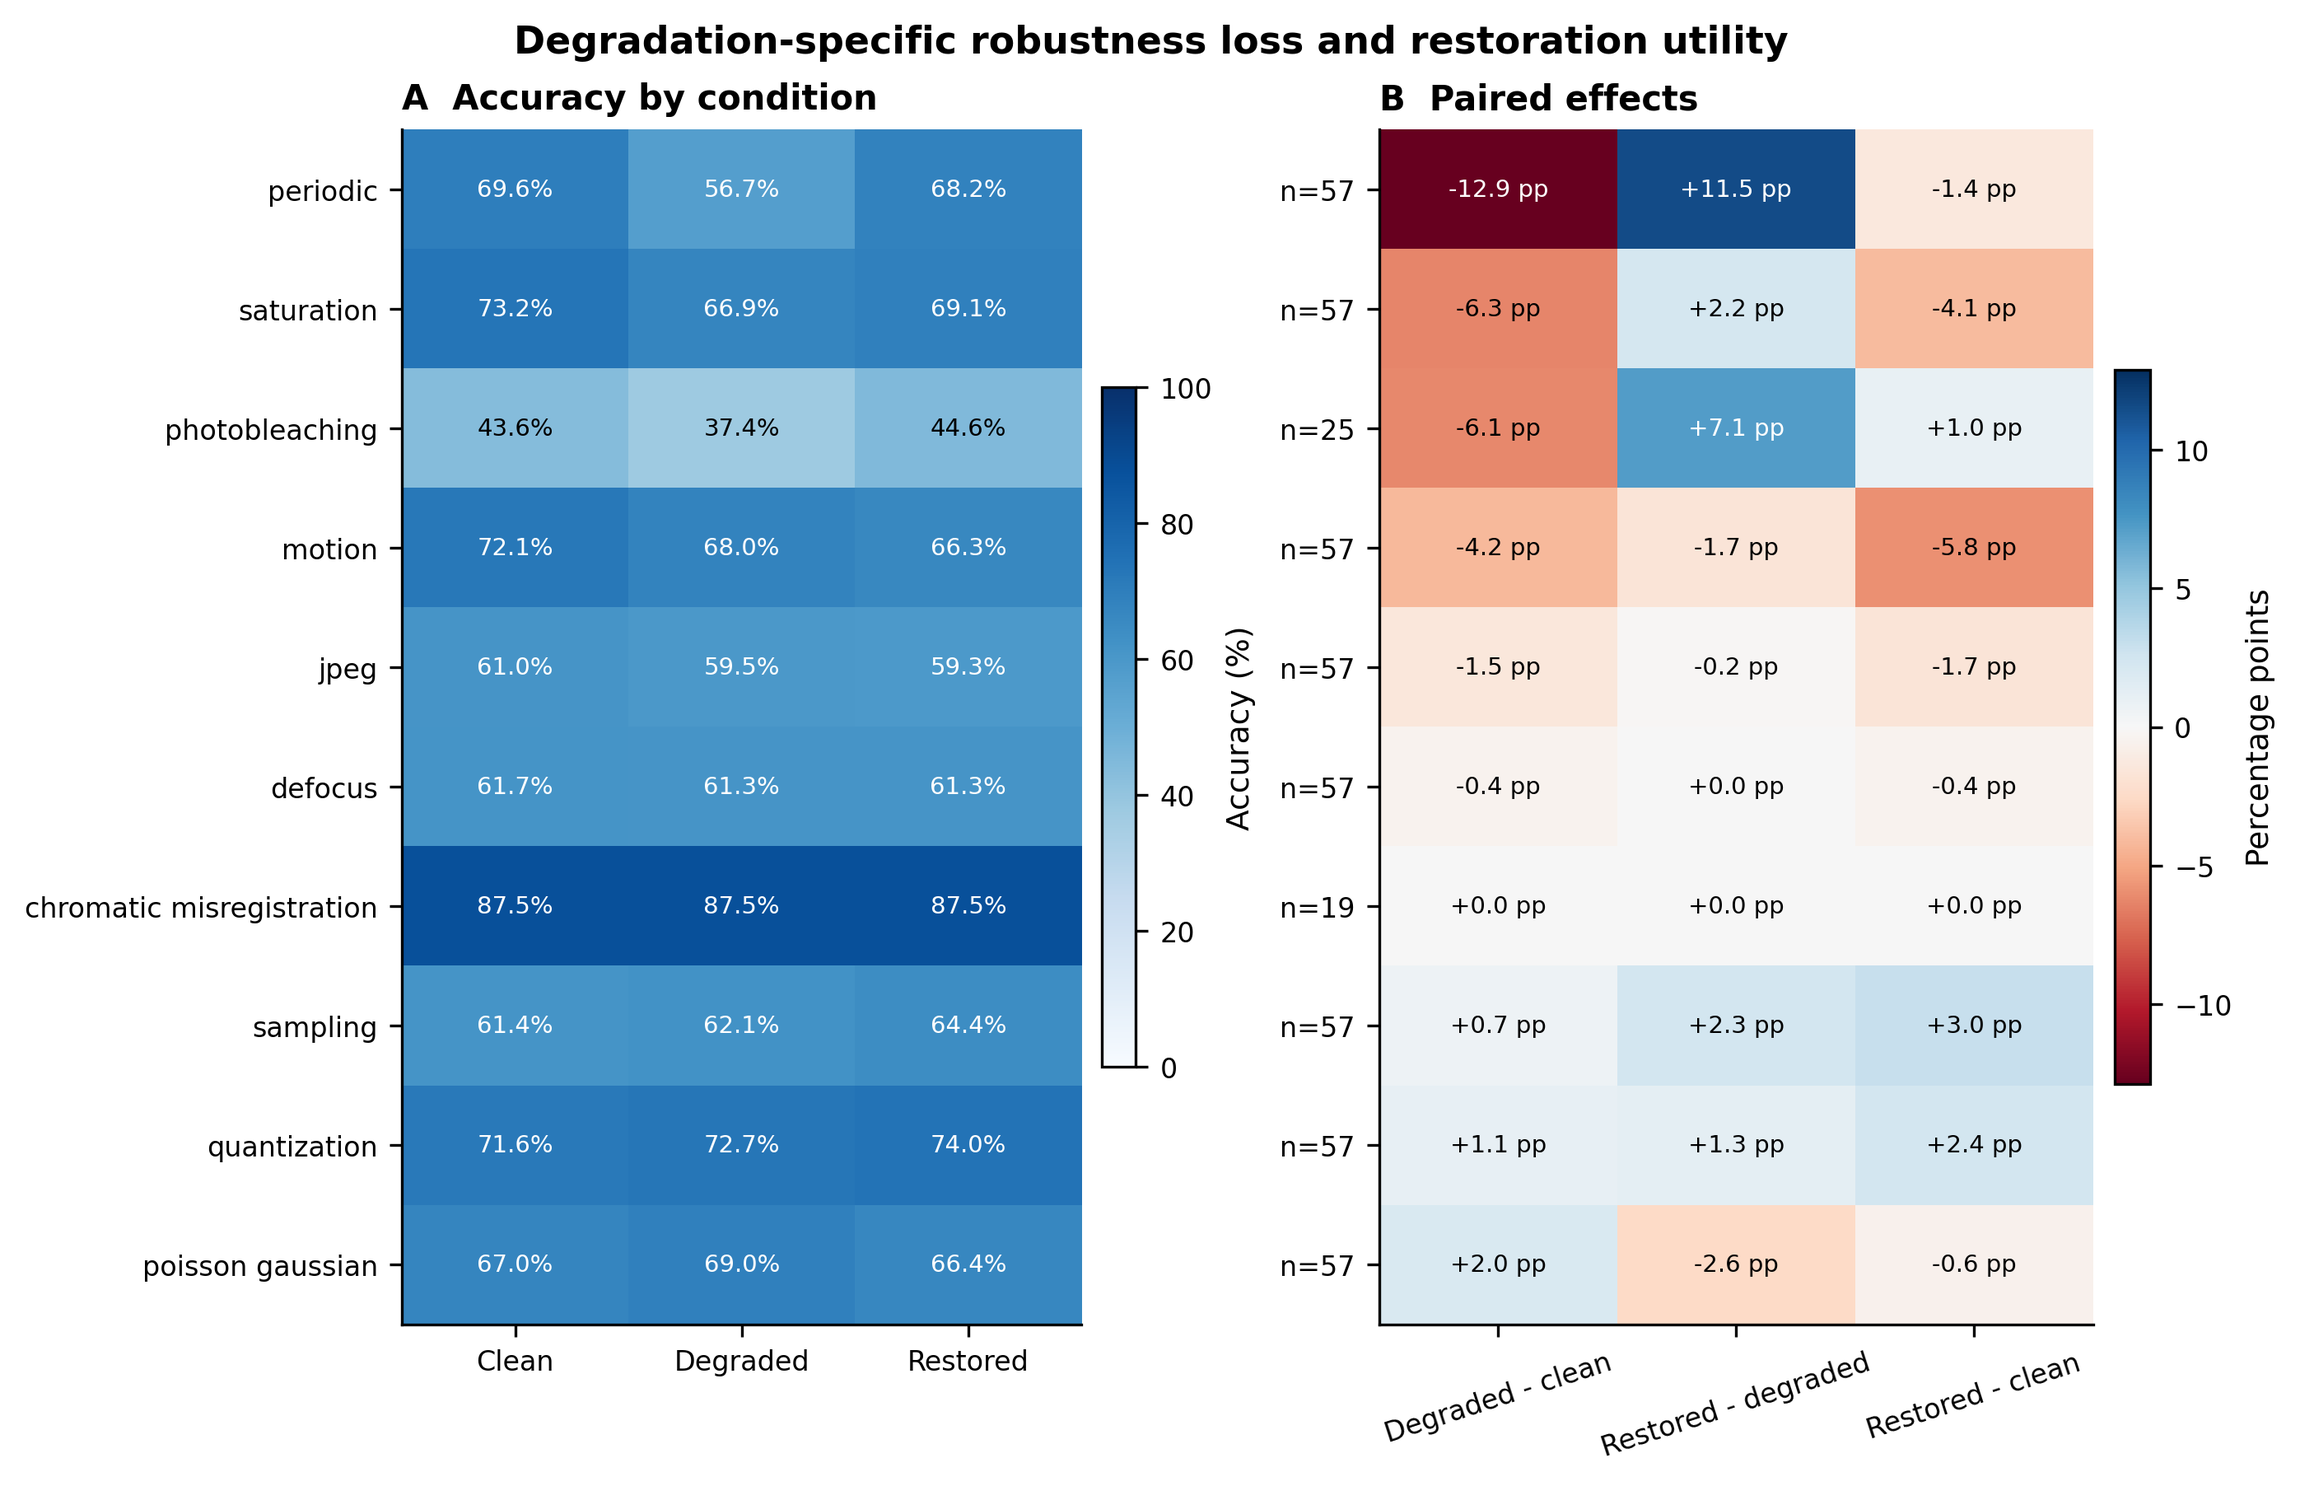
\includegraphics[width=0.95\textwidth]{Figures/robust_2.png}
    \caption{Showing degradation specific robustness and restoration effect on measured accuracies}
\end{figure}

\subsection{Degradation-Specific Response}

Aggregate averages conceal substantial heterogeneity across degradation families
(Table~\ref{tab:vlm_family}). \textbf{Periodic interference} produces by far the largest
robustness loss ($-12.9$~pp, clean$\to$degraded) but is also nearly fully recovered by
restoration ($+11.5$~pp, degraded$\to$restored), leaving only a $-1.4$~pp residual
relative to clean --- mirroring the pixel-level finding that structured, known-frequency
corruption is highly invertible. \textbf{Photobleaching} shows a smaller degradation
loss ($-6.1$~pp) but a comparatively large restoration gain ($+7.1$~pp), i.e.\ gamma/CLAHE
contrast enhancement helps the VLM even though it does not fully restore pixel fidelity.
By contrast, \textbf{motion blur} restoration is actually \emph{harmful} at the semantic
level ($-1.7$~pp degraded$\to$restored, widening the residual to $-5.8$~pp versus clean),
illustrating that a pixel-level restoration success does not guarantee a downstream
semantic benefit. \textbf{Chromatic misregistration} shows no measurable effect in
either direction, and subgroup sample sizes range from $n=19$ to $n=57$, so
family-specific point estimates should be read with appropriate caution.

\begin{table}[h]
\centering
\small
\begin{tabular}{@{}l r r r r r@{}}
\toprule
\textbf{Family} & \textbf{Clean \%} & \textbf{Degraded \%} & \textbf{Restored \%} &
\textbf{Deg.$-$Clean (pp)} & \textbf{Rest.$-$Deg. (pp)} \\
\midrule
Periodic interference & 69.6 & 56.7 & 68.2 & $-12.9$ & $+11.5$ \\
Detector saturation & 73.2 & 66.9 & 69.1 & $-6.3$ & $+2.2$ \\
Photobleaching & 43.6 & 37.4 & 44.6 & $-6.1$ & $+7.1$ \\
Motion / scan drift & 72.1 & 68.0 & 66.3 & $-4.2$ & $-1.7$ \\
JPEG compression & 61.0 & 59.5 & 59.3 & $-1.5$ & $-0.2$ \\
Defocus blur & 61.7 & 61.3 & 61.3 & $-0.4$ & $+0.0$ \\
Chromatic misregistration & 87.5 & 87.5 & 87.5 & $0.0$ & $0.0$ \\
Sampling / resolution loss & 61.4 & 62.1 & 64.4 & $+0.7$ & $+2.3$ \\
Bit-depth quantization & 71.6 & 72.7 & 74.0 & $+1.1$ & $+1.3$ \\
Poisson--Gaussian noise & 67.0 & 69.0 & 66.4 & $+2.0$ & $-2.6$ \\
\bottomrule
\end{tabular}
\caption{Qwen3-VL macro accuracy by degradation family and pixel condition,
subgroup $n$ ranges 19--57. pp = percentage points.}
\label{tab:vlm_family}
\end{table}

\subsection{Severity Response}

Semantic robustness separates most clearly under \textbf{strong} corruption: clean
accuracy of 66.6\% falls to 60.6\% under strong degradation ($-6.0$~pp), and restoration
recovers only $+2.0$~pp, leaving a $-4.0$~pp residual relative to clean. In contrast,
weak and medium severity strata show no consistent accuracy loss, with wide, overlapping
confidence bands. This indicates that the semantic robustness of the model is largely
preserved at low corruption levels and degrades primarily once corruption becomes
severe.

\subsection{Paired Correctness Transitions}

A per-sample transition audit across all 500 unique Micro-Bench samples shows that
\textbf{59.6\%} (298/500) of samples remain correct across all three conditions
(\emph{stable correct}), while \textbf{27.2\%} (136/500) are incorrect under every
condition (\emph{always incorrect}). Restoration \textbf{fixes} 13 samples that were
wrong under degradation, \textbf{misses} 16 samples that remain wrong after
restoration, and actively \textbf{harms} 7 samples that were correct under degradation
but become incorrect after restoration. Splitting by granularity, coarse-perception
questions are stable correct 74\% of the time (17\% always incorrect), while
fine-perception questions are stable correct only 53\% of the time (32\% always
incorrect) --- reinforcing that fine perception is the primary locus of semantic
fragility. A per-family recovery map further shows that periodic interference lies
close to the line of full recovery (robustness loss $\approx$ restoration gain), whereas
motion blur and Poisson--Gaussian noise lie \emph{below} that line, indicating
restoration does not fully offset --- and in the case of motion blur, compounds --- the
semantic damage.

\begin{figure}[h]
    \centering
    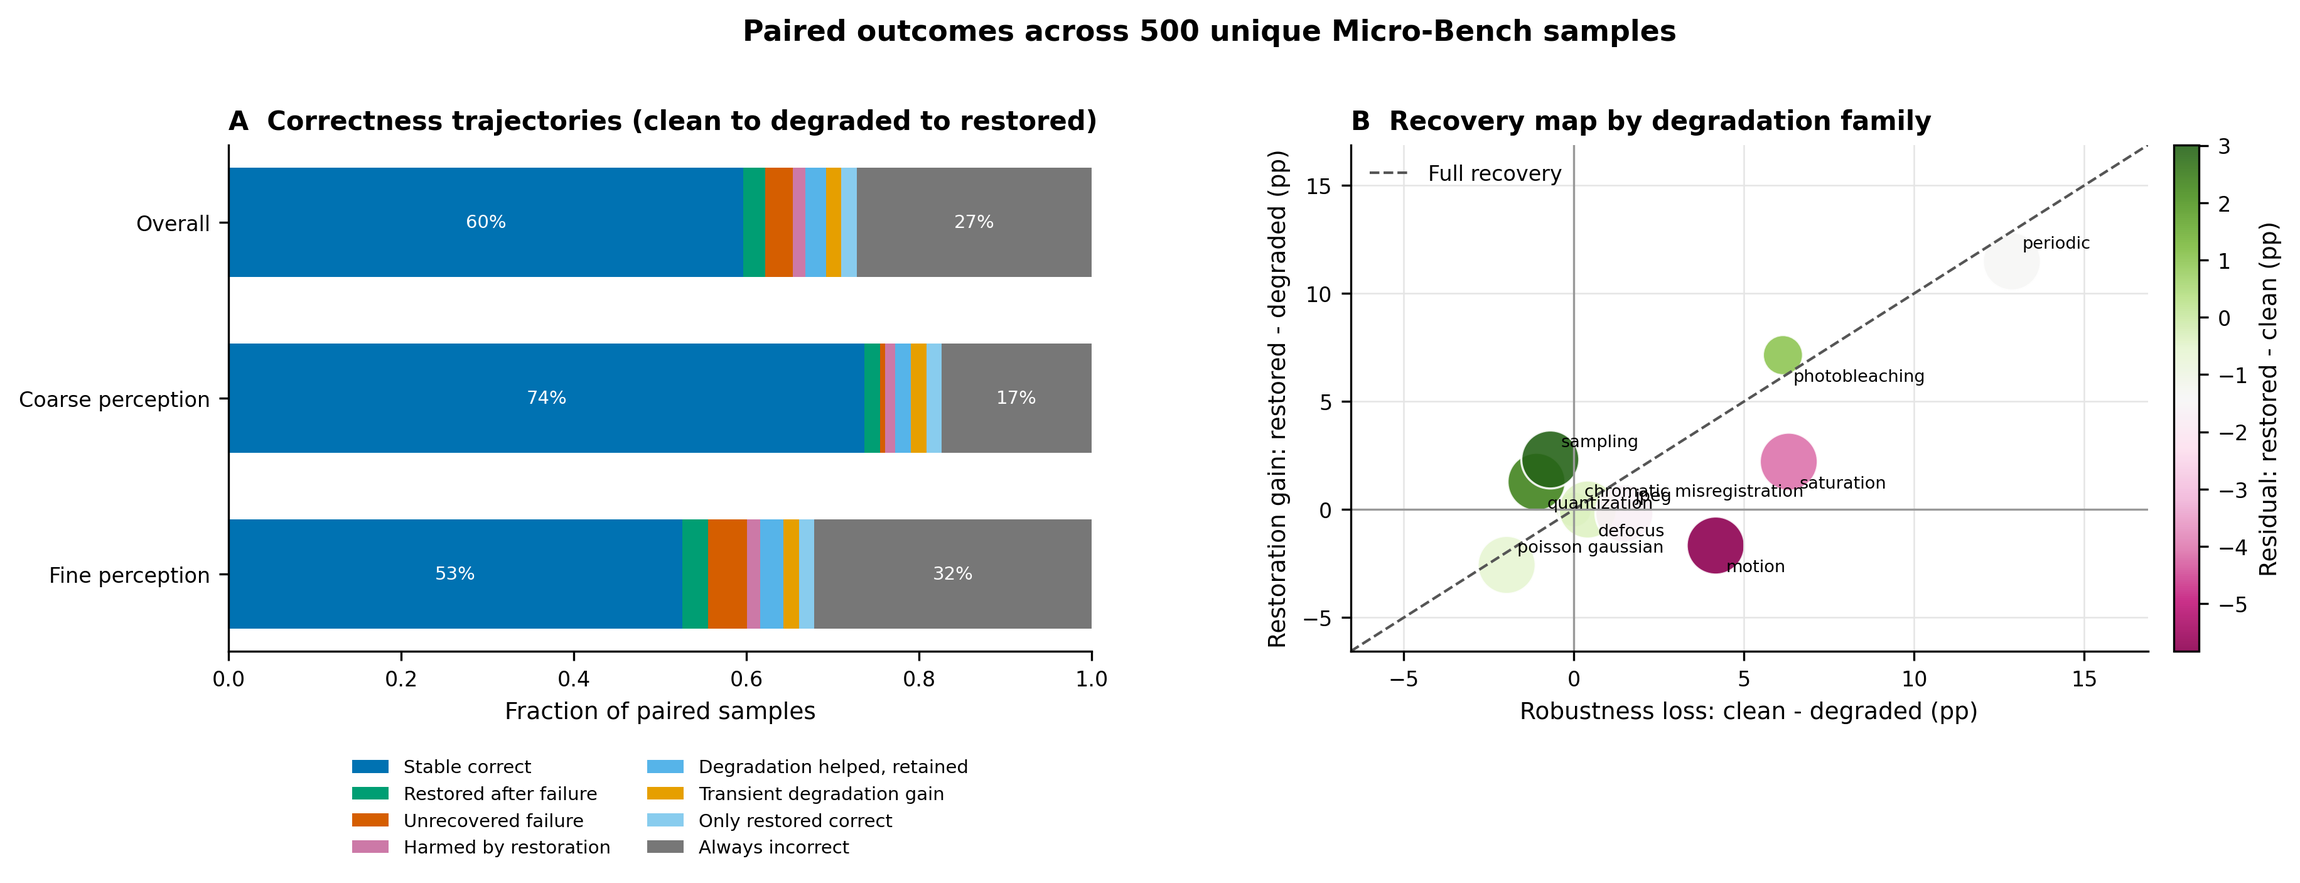
\includegraphics[width=0.95\textwidth]{Figures/robust_4.png}
    \caption{Shows a correctness trajectories regarding how restoration and degradation effected the predicted label. Also recovery map by degradation family is shown here as well.}
\end{figure}

% ============================================================
\section{Discussion and Conclusions}
% ============================================================

Three main conclusions are supported by the combined evidence from Phase 1 and Phase
1.5:

\begin{enumerate}[leftmargin=1.6em]
    \item \textbf{A reproducible classical DIP benchmark.} Starting from 1{,}701 clean
    sources, the pipeline produces 15{,}480 fully provenanced degradation/restoration
    recipes with strict train/evaluation separation, deterministic seeding, and 99.95\%
    empirical severity monotonicity. Zero validation errors or warnings were recorded
    across the full release.
    \item \textbf{Restoration effectiveness follows invertibility, not visual polish.}
    Degradations with a structured, known forward model --- periodic interference,
    Poisson--Gaussian noise, and (partially) motion blur --- are substantially
    recoverable by matched classical restoration at the pixel level. Degradations that
    discard information irreversibly --- quantization, detector saturation, sampling
    loss, photobleaching, and JPEG compression --- remain information-limited, and
    contrast-enhancement-based restoration can even reduce measured pixel fidelity
    while superficially improving visual appearance.
    \item \textbf{Fine-grained perception is the semantic stress point.} The overall
    change in VLM macro accuracy under degradation is modest and statistically
    uncertain at $n=500$, but this aggregate figure conceals large, family- and
    severity-specific effects. Strong corruption and fine-perception question types
    expose meaningful paired failures --- and, notably, pixel-level restoration success
    does not always translate into semantic recovery (e.g.\ motion blur), while in at
    least one case (photobleaching) semantic recovery exceeds what pixel metrics alone
    would predict.
\end{enumerate}

\textbf{Scope and limitations.} All degradations studied here are controlled,
\emph{synthetic} corruptions applied to real microscopy images, rather than corruptions
captured directly from instrument variability; the Phase 1.5 VLM results are exploratory,
based on a single model (Qwen3-VL-8B) and $n=500$ paired samples, several
family-specific subgroups are as small as $n=19$, and improvement in pixel-level fidelity
does not automatically imply improvement in biological or semantic correctness. These
results should therefore be read as evidence of feasibility and direction rather than as
definitive, model-agnostic conclusions.

We close with the open question that motivated this project: \emph{which image
failures should a microscopy-focused vision-language model be trained to notice --- and
when should it instead admit that the underlying information is simply gone?}

% ============================================================
\section*{Acknowledgments}
% ============================================================
This project builds directly on the $\mu$-Bench evaluation benchmark (NeurIPS 2024) and
the low-level vision curricula introduced by Q-Instruct (CVPR 2024) and Q-Bench (ICLR
2024). Training and development pool images are drawn from BBBC010, BBBC038, and
IDR0067, released under CC0 / CC0-1.0 / CC-BY-4.0 / CC-BY-SA-4.0 licenses.

\end{document}
